\subsection{Geometria}

\begin{figure}
	\center
	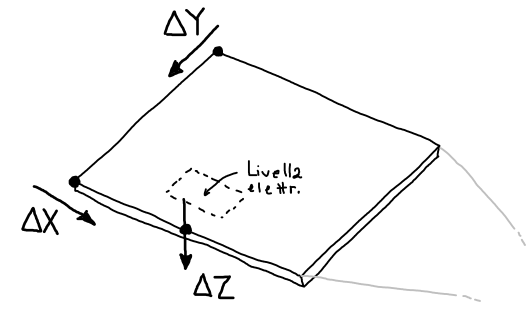
\includegraphics[width=20em]{geometriamis}
	\caption{\label{fig:geometriamis}
	Misura della geometria di una lastra di scintillatore.
	La \emph{profondità} $\Delta Z$ è misurata con il metro a nastro
	con riferimento la lastra più in alto (PM6).
	I \emph{disallineamenti} $\Delta X$ e $\Delta Y$ sono misurati
	con il righello o il metro a nastro usando come riferimento
	una livella a bolla.
	Le \emph{inclinazioni} $\alpha$ e $\beta$ sono misurate con
	una livella elettronica (un telefono) che ha una risoluzione di \SI{0.1}{\degree}.}
\end{figure}

Dobbiamo misurare le caratteristiche gemetriche dell'apparato
per assegnare misure alle variabili del modello in \autoref{fig:geometriadef}.

Con una livella a bolla controlliamo che tutte le lastre siano orizzontali.
La livella a bolla ha, per verifica empirica, una risoluzione minore di quella
elettronica del telefono (\SI{1}{\degree}).
Tuttavia la livella elettronica non ha uno zero fisso; lo zero va impostato
appoggiandola su una superficie di riferimento.
Allora misuriamo l'inclinazione delle lastre (gli angoli $\alpha$ e $\beta$,
che sono gli angoli di Eulero del telefono forniti dal software)
\marginpar{Controllare con il telefono di Bob se sono effettivamente questi angoli
come li sto definendo fin'ora.}
con la livella elettronica, e poi assumiamo, come detto nella \autoref{sec:teogeom},
che l'inclinazione media delle lastre sia nulla.
Questo ci permette di valutare in modo quantitativo quantomeno l'incertezza
dovuta all'inclinazione relativa delle lastre.

Misuriamo la posizione spaziale usando righello, metro a nastro e livella a bolla.
Facendo riferimento alla \autoref{fig:geometriamis} per la notazione,